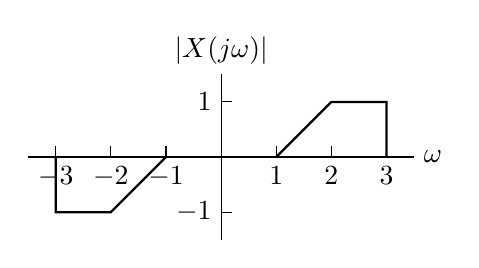
\begin{tikzpicture}[scale=0.70]
	\begin{scope}
		\draw (-3.5,0) -- (3.5,0) node[anchor=west] {$\omega$};
		\draw (0, -1.5) -- (0,1.5) node[anchor=south] {$|X(j\omega)|$};	
		\foreach \x in {-3, -2, -1, 1, 2, 3}
		{
			\draw (\x, 0.2) -- ++(0, -0.2);
			\node at (\x, 0) [anchor=north ] {$\x$};
		}
		\foreach \y in {-1, 1}
		{
			\draw (0.2, \y) -- ++(-0.2, 0);
			\node at (0, \y) [anchor=east ] {$\y$};
		}	
		
		\draw[thick] (-3,0) |- (-2, -1) -- (-1,0) (1,0) -- (2,1) -| (3,0); 
	\end{scope}
	
\end{tikzpicture} 